%%%%%%%%%%%%%%%%%%%%%%%%%%%%%%%%%%%%%%%%%
% TMDEI Dissertation
% LaTeX Template
% Version 0.1 (Dec/2015)
%
% Adapted to TMDEI/ISEP style (Dec/2015) by
%  Nuno Pereira (nap@isep.ipp.pt) and
%  Paulo Baltarejo (pbs@isep.ipp.pt)
%
% Based on MastersDoctoralThesis Version 1.2 by Vel (vel@latextemplates.com) and
% Johannes Böttcher, downloaded from (21/11/15):
% http://www.LaTeXTemplates.com
%
% This template is originally based on a template by:
% Steve Gunn (http://users.ecs.soton.ac.uk/srg/softwaretools/document/templates/)
% Sunil Patel (http://www.sunilpatel.co.uk/thesis-template/)
%
% Template license:
% CC BY-NC-SA 3.0 (http://creativecommons.org/licenses/by-nc-sa/3.0/)
%
%%%%%%%%%%%%%%%%%%%%%%%%%%%%%%%%%%%%%%%%%
%https://www.overleaf.com/project/5bfd7e508cfbf932785021c9
%----------------------------------------------------------------------------------------
%	PACKAGES AND OTHER DOCUMENT CONFIGURATIONS
%----------------------------------------------------------------------------------------

\documentclass[
11pt, % The default document font size, options: 10pt, 11pt, 12pt
oneside, % Two side (alternating margins) for binding by default, uncomment to switch to one side (for drafting/reading purposes)
english, % english for English;
%portuguese,% for Portuguese; delete temporary files if you change language (e.g. 'make clean; make')
singlespacing, % Single line spacing, alternatives: onehalfspacing or doublespacing (for drafting/reading purposes)
%draft, % Uncomment to enable draft mode (no pictures, no links, overfull hboxes indicated)
%nolistspacing, % If the document is onehalfspacing or doublespacing, uncomment this to set spacing in lists to single
liststotoc, % Uncomment to add the list of figures/tables/etc to the table of contents (recommended)
%toctotoc, % Uncomment to add the main table of contents to the table of contents (not recommended)
parskip, % Add space between paragraphs (recommended)
%nohyperref, % Uncomment to not load the hyperref package (not recommended)
nohyperreflinkcolor, % hyperref links are not colored (comment to color links, for example to produce an electronic-only version)
headsepline, % Uncomment to get a line under the header
]{tmdei-style} % The class file specifying the document structure

\usepackage{tikz} % Required for creating graphics programmatically (can be removed if not used)
%\usetikzlibrary{arrows} % Required for fancy arrows in TiKZ graphics (can be removed if not used)

\usepackage{pgfplots} % Required for drawing high--quality function plots (can be removed if not used)
\pgfplotsset{compat=newest}

%
% Next you have examples of admissable citation styles; we recomend using the authoryear-comp citation style (which resembles Harvard); don't forget to only uncomment one
%

% authoryear-comp: recommended citation style (e.g. (Buendía, 1860), (Buendía 1910, Arcadio 1940))
\usepackage[style=numeric-comp,backend=biber]{biblatex} % Bibtex backend with the authoryear-comp citation style (authoryear citations, bibliography ordered alphabetically)

% numeric citation style (e.g. [1], [1-3])
%\usepackage[style=numeric-comp,sorting=none,backend=biber]{biblatex} % Bibtex backend with the numeric-comp citation style (numeric citations, bibliography ordered by appearance)

% alphabetic citation style (e.g. [Buendía10], [Buendía10, Arcadio40])
%\usepackage[style=alphabetic,sorting=none,backend=biber]{biblatex} % Bibtex backend with the alphabetic citation style (alphabetic citations, bibliography ordered by appearance)
\usepackage{macros}

\addbibresource{mainbibliography.bib} % The filename of the bibliography

\makeglossaries % build the glossary

%----------------------------------------------------------------------------------------
%	THESIS INFORMATION
%----------------------------------------------------------------------------------------

\thesistitle{Feedback Linearizable Discretization \\ \vspace{5pt} of Second-Order Mechanical Systems \vspace{2pt} using Retraction Maps} % Your thesis title, this is used in the title, print it elsewhere with \ttitle

%\thesissubtitle{{[}Thesis Subtitle{]}} % Your thesis title, this is used in the title, print it elsewhere with \tsubtitle

\author{Shreyas \textsc{N B}} % Your name, this is used in the title page, print it elsewhere with \authorname

\subjectarea{Systems and Controls Engineering} % Specialisation area (Computer Systems, Information and Knowledge Systems, Graphics, Systems and Multimedia, Software Engineering), used in the title page, print it elsewhere with \areaname

\supervisor{Prof.~Ravi \textsc{Banavar}} % Your advisors's name, this is used in the title page, print it elsewhere with \supname

\cosupervisor{Prof.~Krishnendu \textsc{Haldar}} % Your co-advisors's name, this is used in the title page, print it elsewhere with \cosupname (comment, if no co-supervisor)

% if committeepresident is defined, will add the thesis committee to the front page
%\committeepresident{Dr. Jonny Smith, Professor, DEI/ISEP} % Name of the president of the evaluation committee, print it elsewhere with \presidentname

%\committeemembers{Dr. Jaimie Smith, Professor, DEI/ISEP\\Dr. Jones Smith, Professor, DEI/ISEP\\Dr. Jagger Smith, Professor, DEI/ISEP} % Name of the evaluation committee members (up to four), print it elsewhere with \committee

\keywords{geometric integrators, retraction maps, discrete systems, feedback linearization, mechanical systems} % Please define up to 6 keywords that better describe your work, print it elsewhere with \keywordnames

\university{Indian Institute of Technology, Bombay} % Your university's name and URL, this is used in the title page and abstract, print it elsewhere with \univname

\department{Department of Aerospace Engineering} % Your department's name and URL, this is used in the title page and abstract, print it elsewhere with \deptname

\thesisdate{\today} % thesis date,  print it elsewhere with \tdate

\hypersetup{pdftitle=\ttitle} % Set the PDF's title to your title
\hypersetup{pdfauthor=\authorname} % Set the PDF's author to your name
\hypersetup{pdfkeywords=\keywordnames} % Set the PDF's keywords to your keywords

\begin{document}

%----------------------------------------------------------------------------------------
%	FRONT MATTER
%----------------------------------------------------------------------------------------

% Include the frontmatter of your thesis here
% we include the glossary here (frontmatter is included with \input, so this command is as if it was in main.tex)
%All acronyms must be written in this file.
\newacronym{RTS}{RTS}{Real-Time System}
\newacronym{GPOS}{GPOS}{General Purpose Operating System}
\newacronym{RTOS}{RTOS}{Real-Time Operating System}
\newacronym{PGF}{PGF}{Portable Graphics Format}


\frontmatter % Use roman page numbering style (i, ii, iii, iv...) for the pre-content pages

\pagestyle{plain} % Default to the plain heading style until the thesis style is called for the body content

%----------------------------------------------------------------------------------------
%	TITLE PAGE
%----------------------------------------------------------------------------------------

\maketitlepage


%----------------------------------------------------------------------------------------
%	STATEMENT of INTEGRITY
%----------------------------------------------------------------------------------------
\integritystatement%

%----------------------------------------------------------------------------------------
%	DEDICATION  (optional)
%----------------------------------------------------------------------------------------
%
%\dedicatory{For/Dedicated to/To my\ldots}
% \begin{dedicatory}
% The dedicatory is optional. Below is an example of a humorous dedication.

% "To my wife Marganit and my children Ella Rose and Daniel Adam without whom this book would have been completed two years earlier." in "An Introduction To Algebraic Topology" by Joseph J. Rotman.
% \end{dedicatory}

%----------------------------------------------------------------------------------------
%	ABSTRACT PAGE
%----------------------------------------------------------------------------------------

\begin{abstract}

% here you put the abstract in the main language of the work.

Mechanical systems are most often described by a set of continuous-time, nonlinear, second-order differential equations (SODEs) of a particular structure governed by the covariant derivative. The digital implementation of controllers for such systems requires a discrete model of the system and hence requires numerical discretization schemes. Feedback linearizability of such sampled systems, however, depends on the discretization scheme employed. \\\\ In this thesis, we utilize retraction maps and their lifts to construct feedback linearizable discretizations for SODEs which can be applied to many mechanical systems.

\end{abstract}


%----------------------------------------------------------------------------------------
%	ACKNOWLEDGEMENTS (optional)
%----------------------------------------------------------------------------------------

\begin{acknowledgements}

I would like to thank Prof.~David M. Diego, Insituto de Ciencias Matemáticas (ICMAT), for his guidance in the development of the theory in this document.

I would also like to acknowledge the support of my family, friends, and colleagues, who have supported me throughout the development of this work.

\end{acknowledgements}

%----------------------------------------------------------------------------------------
%	LIST OF CONTENTS/FIGURES/TABLES PAGES
%----------------------------------------------------------------------------------------

\tableofcontents % Prints the main table of contents

\listoffigures % Prints the list of figures

\listoftables % Prints the list of tables

\listofalgorithms % Prints the list of algorithms
\addchaptertocentry{\listalgorithmname}


\renewcommand{\lstlistlistingname}{List of Source Code}
\lstlistoflistings % Prints the list of listings (programming language source code)
\addchaptertocentry{\lstlistlistingname}


%----------------------------------------------------------------------------------------
%	ABBREVIATIONS
%----------------------------------------------------------------------------------------
%\begin{abbreviations}{ll} % Include a list of abbreviations (a table of two columns)
%%\textbf{LAH} & \textbf{L}ist \textbf{A}bbreviations \textbf{H}ere\\
%%\textbf{WSF} & \textbf{W}hat (it) \textbf{S}tands \textbf{F}or\\
%\end{abbreviations}

%----------------------------------------------------------------------------------------
%	SYMBOLS
%----------------------------------------------------------------------------------------

\begin{symbols}{ll} % Include a list of Symbols (a two column table)

$\mathcal{R}$ & retraction map \\
$\mathcal{D}$ & discretization map \\
%Symbol & Name & Unit \\

\end{symbols}



%----------------------------------------------------------------------------------------
%	ACRONYMS
%----------------------------------------------------------------------------------------

\newcommand{\listacronymname}{List of Acronyms}

%Use GLS
\glsresetall
\printglossary[title=\listacronymname,type=\acronymtype,style=long]

%----------------------------------------------------------------------------------------
%	DONE
%----------------------------------------------------------------------------------------

\mainmatter % Begin numeric (1,2,3...) page numbering
\pagestyle{thesis} % Return the page headers back to the "thesis" style


%----------------------------------------------------------------------------------------
%	MAIN BODY
%----------------------------------------------------------------------------------------

% Include the chapters of the thesis as separate folder for each chapter
% Uncomment the lines as you write the chapters

% Chapter 1
% 
\chapter{Retraction Maps} % Main chapter title
\label{chap:retr} % For referencing the chapter elsewhere, use Chapter~\ref{Chapter1}


%-------------------------------------------------------------------------------
%---------
%
\section{Introduction} 
\label{sec:retr-intro} %For referencing this section elsewhere, use Section~\ref{sec:chap1_introduction}

The notion of a retraction map is fundamental in research areas like optimization theory, machine learning, numerical analysis, and in this context, geometric integrators. \\ Many mechanical systems usually evolve on manifolds, which naturally requires some method of discretely approximating the dynamics on the manifold (i.e., the geodesic). 

In Riemannian geometry, this idea is given by the exponential map. On a Riemannian manifold $(M, g)$, we define $\exp: T_x M \lra M$ as the exponential map at the point $x$. For instance, if  $\gamma: [0, 1] \lra M$ is a unique geodesic on $M$, and $\gamma(0) = x$, then $\exp_x(v) = \gamma(1)$, where $v \in T_x M$ is the initial velocity of the geodesic at $x$ such that $\dot{\gamma}(0) = v$.

    \begin{figure}[h]
        \centering
        \scalebox{0.8}{
           \begin{tikzpicture}[
          point/.style = {draw, circle, fill=black, inner sep=1.4pt}
        ]
                \draw[fill=green!15, draw=black, shift={(0.4, 1.4)},scale=1.5] (0, 0) to[out=20, in=140] (3, -0.4) to [out=60, in=160] (10, 1) to[out=130, in=60]
          cycle;
        \filldraw[xslant=-0.5, fill=gray!60, opacity=0.25]
          (8,7) -- (16,7) -- (16,3) -- (8,3) -- cycle; 
          \node at (11.6, 6) {$T_x M$};
          \node at (2,2.4) {$M$};
          \node at (10, 5) {$x = \gamma(0)$};
          \node[red] at (7, 5) {$v = \dot{\gamma}(0)$};
          \node[blue] at (4.5, 3) {$\Ret_x(v)$};
          \node[black] at (6.8, 3.7) {$\gamma(t)$};
          \coordinate (X) at (9,4.9);
          \coordinate (O) at (5.4,4.4);
          \coordinate (P) at (5.4,2.4);
            \node[point] at (X) {};
          \node[point] at (P) {};
          \draw[thick, dashed] (5.5, 2.7) arc (153:92:4);
          \draw[blue, -{Latex[length=4mm]}] (O) -- (P);
          \draw[red, -{Latex[length=4mm]}] (X) -- (O);
        \end{tikzpicture}}
        \caption{Retraction maps: A visualization}
            \label{fig:retraction}
        \end{figure}

Let $M$ be an $n$ dimensional manifold, and $TM$ be its tangent bundle.

\begin{defn}\label{defn:retraction}
We define a \textbf{retraction map} on a manifold $M$ as a smooth map $\Ret: TM \to M$, such that if $\Ret_x$ be the restriction of $\Ret$ to $T_x M$, then the following properties are satisfied:

    \begin{enumerate}
        \item $\Ret_x (0_x) = x$ where $0_x$ is the zero element of $T_x M$.
        \item $\text{D}\Ret_x (0_x ) = T_{0_x} \Ret_x = \text{Id}_{T_x M} $, where $\text{Id}_{T_x M}$ is the identity mapping on $T_x M$.
    \end{enumerate}
\end{defn}

Here, the first property is trivial, whereas the second property is known as the \textbf{local rigidity condition} since, given $v \in T_x M$, the curve $\gamma_v(t) = \Ret_x(tv)$ has initial velocity $v$ at $x$. Hence,

\[
  \dot{\gamma}_v (t) = \langle \text{D}\Ret_x (tv) , v \rangle \implies \dot{\gamma}_v (0) = \text{Id}_{T_x M}(v) = v
\]

\section{Discretization maps}

\begin{defn}
A map $\D : U \subset TM \lra M \times M$ given by 

\[
  \D (x,v) = \left( \Ret^1_x(v), \Ret^2_x(v) \right)
\]

where $U$ is the open neighborhood of the zero section $0_x \in TM$, is called a \textbf{discretization map} on $M$, if the following properties are satisfied:

\begin{enumerate}
  \item $\D(x,0_x) = (x,x)$ 
  \item $T_{0_x}\Ret_x^2 - T_{0_x}\Ret_x^1 = \text{Id}_{T_x M}$, which is the identity map on $T_x M$ for any $x \in M$.
\end{enumerate}
\end{defn}

Using this definition, one can prove (not included here) that the discretization map $\D$ is a local diffeomorphism around the zero section $0_x \in TM$. This is a crucial property for the construction of geometric integrators, since we need to be able to define $\D^{-1} (x_k, x_{k+1})$.

Thus, given a vector field $X \in \mathfrak{X}(M)$ on $M$, i.e., $X: M \lra TM$ such that $\tau_M \circ X = \text{Id}_M$, where $\tau_M: TM \lra M$ is the canonical projection on the tangent bundle, we can approximate the integral curve by the following first-order discrete equation:

\[
  h X(\tau_M(\D^{-1}(x_k, x_{k+1}))) = \D^{-1}(x_k, x_{k+1})
\]

Hence, given an initial condition $x_0$, we may be able to solve the discrete equation iteratively to obtain the sequence $\{x_k\}$ which is indeed an approximation of $\{x(kh)\}$, where $x(t)$ is the integral curve of $X$ with initial condition $x_0$ and time-step $h$.

\subsection{Examples}
We consider a few examples of discretization maps on $\R[n]$:

\begin{table}[h]
\centering
\begin{tabular}{|c|c|c|}
\hline
 Discretization map $\D$ & Scheme & Order \\
\hline
 $\D(x,v) = (x, x + v)$ & Forward Euler $x_{k+1} = x_k + hX(x_k)$ & $\mathcal{O}(h)$ \\
 $\D(x,v) = (x - v, x)$ & Backward Euler $x_k = x_{k+1} - hX(x_{k+1})$ & $\mathcal{O}(h)$\\
 $\D(x, v) = \left(x - \dfrac{v}{2}, x + \dfrac{v}{2} \right)$ & Symmetric Euler $x_{k+1} = x_k + hX\left( \dfrac{x_k + x_{k+1}}{2}\right)$ & $\mathcal{O}(h^2)$\\
\hline
\end{tabular}
\caption{Examples of discretization maps}
\end{table}


\section{Lifts of discretization maps}

As mentioned before, discretization maps are diffeomorphisms around the zero section $0_x \in TM$. 
This is useful because typically when studying mechanical systems, we would like to define the discretization map on the tangent bundle $TM$ (for Lagrangian frameworks) or the cotangent bundle $T^*M$ (for Hamiltonian frameworks), in order to generate geometric integrators on the manifold.

Thus, since discretization maps can be defined on different manifolds, we denote $\D^{TM} : TM \lra M \times M$ as a discretization map on $M$.

\subsection{Tangent Lifts of Discretization Maps}

Given a smooth map $\varphi: M \lra N$ between two $n$-dimenstional manifolds $M$ and $N$, we can define the \textbf{tangent lift} of $\varphi$ as the map $T\varphi: TM \lra TN$ such that

\[
  T\varphi(v_x) = T_x \varphi(v_x) \in T_{\varphi(x)} N
\]

where $v_x \in T_x M$ and $T_x\varphi$ is the tangent map of $\varphi$, whose matrix is the Jacobian at $x \in M$, in a local chart.

\begin{prop}
Let $M$ and $N$ be two $n$-dimensional manifolds, and $\varphi: M \lra N$ be a smooth map (diffeomorphism). For a given discretization map $\D^{TM}$ on $M$, the map $\D_{\varphi} :=  (\varphi \times \varphi) \circ \D^{TM} \circ T \varphi ^{-1}$ is a discretization map on $N$ i.e., $\D_{\varphi} \equiv \D^{TN} : TN \lra N \times N$.
\end{prop}


\begin{proof}
  For any given $y \in N$, we have that 
  \begin{equation*}
    \begin{split}
      \D_{\varphi} (y, 0_y) &= ((\varphi \times \varphi) \circ \D^{TM} \circ T\varphi^{-1}) (y, 0_y) \\
      &= ((\varphi \times \varphi) \circ \D^{TM} \circ T\varphi^{-1}) (\varphi(x), 0_{\varphi(x)}) \\
      &= (\varphi \times \varphi) \circ \D^{TM} (x, 0_x) \\ 
      &= (\varphi \times \varphi) (x, x) = (y, y)
    \end{split}
  \end{equation*}

  which proves the first condition. For the second condition, let $v_y \in T_y N$, be a given vector.
  \begin{equation*}
    \begin{split}
      (T_{0_x} \Ret_{x, \varphi}^2 - & T_{0_x} \Ret_{x, \varphi}^1 )(y, u_y) = \dfrac{d}{ds} \bigg{|}_{s=0} \left( \Ret_{x, \varphi}^2 (y, su_y) - \Ret_{x, \varphi}^1 (y, su_y) \right) \\
      &= \dfrac{d}{ds} \bigg{|}_{s=0} \left(\varphi \circ \Ret^1_x \circ T\varphi^{-1} (y, su_y) \right) -  \left( \varphi \circ \Ret^2_x \circ T \varphi^{-1}(y, su_y) \right) \\
      &= T_y \varphi \left( \dfrac{d}{ds} \bigg{|}_{s=0} \left[ \Ret^1_x(t(T\varphi^{-1} (y, u_y))) \right] - \left[ \Ret^2_x(t(T\varphi^{-1} (y, u_y))) \right] \right) \\
      &= T_y \varphi (T_y \varphi^{-1} (y, u_y)) = (y, u_y)
    \end{split}
  \end{equation*}

Thus, both the conditions from Definition~\ref{defn:retraction} are satisfied.
\end{proof}

The above proposition can be visualized as shown below in Figure~\ref{fig:commutator}.

\begin{figure}[h]
  \centering
  \begin{tikzpicture}
\matrix (m) [matrix of math nodes,row sep=3em,column sep=4em,minimum width=2em]
{
   TM & TN \\ M \times M & N \times N \\};
\path[-stealth]
  (m-1-1) edge node [above] {$T\varphi$} (m-1-2)
  (m-1-1) edge node [left] {$\D^{TM}$} (m-2-1)
  (m-1-2) edge node [right] {$\D^{TN}$} (m-2-2)
  (m-2-1) edge node [below] {$\varphi \times \varphi$} (m-2-2);
\end{tikzpicture}
  \caption{$\D^{TM}$ and $\D^{TN}$ commute as shown}
  \label{fig:commutator}
\end{figure}

Now, if we suitably lift the discretization map $\D : TM \lra M \times M$, we can get a discretization map on $TM$, i.e., we can define $\D^{TTM} : TTM \lra TM \times TM$ as a discretization map on $TM$. This construction will provide the geometric framework for integrators for second-order differential equations (SODEs) on manifolds, and consequently, for mechanical systems.

Let $M$ be an $n$-dimensional manifold, and $\tau_M : TM \lra M$ be the canonical projection on the tangent bundle. We denote $TTM$ as the \textbf{double tangent bundle} of $M$.

We note that the manifold $TTM$ naturally accepts two different vector bundle structures:

\begin{enumerate}
  \item The canonical vector bundle with projection $\tau_{TM} : TTM \lra TM$.
  \item The vector bundle given by the projection of the tangent map $T \tau_M : TTM \lra TM$. 
\end{enumerate}

Thus, we denote the canonical involution map $\kappa_M : TTM \lra TTM$ which is a vector bundle isomorphism, over the identity of $TM$ between the above two vector bundle structures.

This can be seen here: Let $(x,v)$ be the canonical coordinates on $TM$, and $(x, v, \dot{x}, \dot{v})$ are the corresponding canonical fibered coordinates on $TTM$. Then,

\[
 \kappa_M (x, v, \dot{x}, \dot{v}) = (x,\dot{x}, v, \dot{v})
\]

\begin{rmk}{Why do we need this?}
  Remember that the tangent lift of a vector field $X$ on $M$ does not define a vector field on $TM$. It is necessary to consider the composition $\kappa_M \circ TX$ to obtain a vector field on $TM$, and this is called the \textbf{complete lift} $X^c$ of the vector field $X$. 
  Hence, a similar technique must be used to lift a discretization map from $TM$ to $TTM$.
\end{rmk}

\begin{figure}[h]
  \centering
  \begin{tikzpicture}[transform shape]
\matrix (m) [matrix of math nodes,row sep=3em,column sep=5em,minimum width=0.1em]
{
   TTM & TM \times TM \\ TTM & T(M \times M) \\ TM & M \times M \\};
\path[-stealth]
    (m-1-1) edge node [above] {$\D^{TTM}$} (m-1-2)
    (m-2-1) edge node [above] {$T \D^{TM}$} (m-2-2)
    (m-2-1) edge node [left] {$\tau_{TM}$} (m-3-1)
    (m-2-2) edge node [right] {$\tau_{M \times M}$} (m-3-2)
    (m-3-1) edge node [above] {$\D^{TM}$} (m-3-2); 
\path[<->]
    (m-1-1) edge node [left] {$\kappa_M$} (m-2-1)
    (m-2-1) edge node [right] {$\kappa_M$} (m-1-1);
\draw[double]
    (m-1-2) -- (m-2-2);
\end{tikzpicture}
  \caption{Tangent lift structure of discretization maps}
  \label{fig:tangent-lift}
\end{figure}

Using the above construction, we can now define the tangent lift of a discretization map.

\begin{prop}
  If $\D^{TM} : TM \lra M \times M$ is a discretization map on $M$, then the map defined by $\D^{TTM} = T\D^{TM} \circ \kappa_M$ is a discretization map on $TM$.
\end{prop}

\begin{proof}
  For $(x,v,\dot{x}, \dot{v}) \in TTM$, we have that 
  
  \[T\D^{TM}(x,v,\dot{x}, \dot{v}) = \left( \D^{TM}(x,v), D_{(x,v)} \D^{TM}(x,v) {(\dot{x}, \dot{v})}^T \right)\] and
  \[
    \D^{TTM}(x, \dot{x}, v, \dot{v}) = (\D^{TM}(x,v), D_{(x,v)}\D^{TM}{(\dot{x}, \dot{v})}^T) 
  \]

  Using the properties defined in Definition~\eqref{defn:retraction},  
  \begin{enumerate}
      \item We know that $\D^{TM}(x, 0) = (x,x) \ \forall x \in M$. Thus,
      \begin{equation*}
      \begin{split}
          \D^{TTM}(x,\dot{x}, 0, 0) & = \left( \D^{TM}(x, 0), D_{(x,0)} \D^{TM}(\dot{x}, 0) \right) \\
          & = (x,x, \dot{x}, \dot{x}) \equiv (x, \dot{x}, x, \dot{x})
      \end{split}
      \end{equation*}
       
      where we trivially identify $T(M \times M) \equiv TM \times TM$.
      \item For the rigidity property, we know that
      \[\D^{TTM}(x, \dot{x}, v, \dot{v}) = \left({(T\Ret^1)}_{(x,\dot{x})}(v, \dot{v}), {(T\Ret^2)}_{(x,\dot{x})}(v, \dot{v}) \right)\]
      So, we need to compute 
      \[T_{{(0,0)}_{(x,\dot{x})}}{(T\Ret^a)}_{(x, \dot{x})}(x, \dot{x}) : T_{(x, \dot{x})}TM \lra T_{(x, \dot{x})}TM\]
      for $a=1,2$, to prove that the map ${T(T\Ret^2)}_{(x,\dot{x})} - T(T\Ret^1)_{(x, \dot{x})}$ is the identity map at the zero section $(0,0)_{(x,\dot{x})}$, from $T_{(x, \dot{x})} TM$ to itself.

      We can calculate 
          \[\dfrac{d}{ds}\bigg|_{s=0} \left( \Ret^a_x( sv), \partial_{x} \Ret^a_x(sv) \dot{x} + \partial_v \Ret^a_x(sv) s \dot{v} \right)\]
      
      At $(x, \dot{x}, 0, 0)$, the map $T_{(0,0)_{(x, \dot{x})}}(T\Ret^a)_{(x, \dot{x})}$ is thus given by:
      \[\pmat{
      \partial_{v^j}(\Ret^a)^i(x, 0) & 0 \\
      \partial_{x^k} \partial_{v^j} (\Ret^a)^i(x,0) \dot{x}^k & \partial_{v^j}(\Ret^a)^i(x,0)
      }\]
      
      \vspace{-1mm}
      Thus, using the properties of the discretization map $\D$, we have the Jacobian matrix of $(T\Ret^2)_{(x, \dot{x})} - (T\Ret^1)_{(x, \dot{x})}$ at $(0,0)_{(x, \dot{x})}$ as:
      \[\pmat{
      \partial_{v}(\Ret^2-\Ret^1)(x,0) & 0 \\
      \partial_x(\partial_v(\Ret^2 - \Ret^1)(x,0))\dot{x} & \partial_v (\Ret^2-\Ret^1)(x,0)
      }
      \]

      \vspace{-1mm}
      which is indeed equal to the identity $\text{ Id}_{2n \times 2n}$, since $\partial_v (\Ret^2-\Ret^1)(x,0) = \text{ Id}_{n \times n}$ which also implies $\partial_x(\partial_v(\Ret^2 - \Ret^1))(x,0) = 0$
  \end{enumerate}
\end{proof}

\subsection{Example}

Let us consider the midpoint rule as an example. Thus, if $M$ is a vector space, $\D : TM \lra M \times M$ is the discretization map given by $\D(x,v) = \left( x - \frac{1}{2}v, x + \frac{1}{2}v \right)$. We can also compute the inverse map as $\D^{-1}(x_k, x_{k+1}) = \left(\dfrac{x_k + x_{k+1}}{2}, x_{k+1} - x_k \right)$.

\newpage

To define the tangent lift of $\D$, denoted by $\D^{TTM}: TTM \lra TM \times TM$, we need to compute the Jacobian of $\D$,

\[
  D_{(x,v)} \D = \pmat{ \text{Id} & -\dfrac{1}{2} \text{Id} \\ \text{Id} & \dfrac{1}{2} \text{Id}}
\]
which yields the tangent lift of $\D$ as:

\begin{equation*}
  \begin{split}
    \D^{TTM} (x, \dot{x}, v, \dot{v}) &= (T\D \circ \kappa_M)\left( x, \dot{x}, v, \dot{v} \right) = T\D(x, v ; \dot{x}, \dot{v}) \\
    &= \left( x - \dfrac{1}{2}v, x + \dfrac{1}{2}v ; \dot{x} - \dfrac{1}{2}\dot{v}, \dot{x} + \dfrac{1}{2} \dot{v} \right) \\
    & \equiv \left( x - \dfrac{1}{2}v, \dot{x} - \dfrac{1}{2}\dot{v} ; x + \dfrac{1}{2}v, \dot{x} + \dfrac{1}{2} \dot{v} \right)
  \end{split}
\end{equation*}

We can also obtain the inverse map of $\D^{TTM}$ as 

\[ {\left(\D^{TTM}\right)}^{-1} (x_k, v_k; x_{k+1}, v_{k+1}) = \left( \dfrac{x_k + x_{k+1}}{2}, \dfrac{v_k + v_{k+1}}{2}; x_{k+1} - x_k, v_{k+1} - v_k \right) \]

% Chapter 2

\chapter{Mechanical Control Systems} % Main chapter title

\label{chap:sode} % For referencing the chapter elsewhere, use \ref{chap:Chapter2} 

Mechanical systems are usually described by nonlinear second-order differential equations (SODEs). In this chapter, we will discuss the geometric formulation of SODEs and their discretization. We will define different classes of mechanical systems, and how a specific class of mechanical systems can be controlled using a technique called \textit{feedback linearization}.

%----------------------------------------------------------------------------------------
\section{Second-order differential equations (SODEs)} 
Let $x \in M$ and $(x, \dot{x}) \in TM$ be the coordinates on the manifold $M$ and the induced coordinates on the tangent bundle of $M$, respectively. We know that a second-order differential equation is a vector field $X$ such that $\tau_{TM}(X) = T \tau_M (X)$. This implies that the vector field $X$ on $TM$ is a section of the second-order tangent bundle $TTM$. Locally, if we take coordinates $(x^i)$ on $M$ and induced coordinates $(x^i, \dot{x}^i)$ on $TM$, then:
\begin{equation}
    X = \dot{x}^i \frac{\partial}{\partial x^i} + X^i(x^i, \dot{x}^i) \frac{\partial}{\partial \dot{x}^i}
\end{equation}
To find the integral curves of $X$ is equivalent to solving the SODE:
\begin{equation}
\label{eq:sode}
    \dfrac{d^2}{dt^2}x(t) = X \left( x(t), \dfrac{d}{dt}x(t) \right) 
\end{equation}
Now, we wish to discretize this using the notion of the discretization map on $TM$. We would like to tangently lift a discretization on $M$ to obtain $\D^{TTM}: TTM \lra TM \times TM$ as defined in Proposition \ref{prop:lift-commutator}. This yields the following numerical scheme [\cite{21MBLDMdD}]:
\begin{equation}
\label{eq:disc}
\begin{split}
    h X \left( \left(\tau_{TM} \circ \left(\D^{TTM}\right)^{-1}\right)(x_k, y_k; x_{k+1}, y_{k+1})\right) \\ = \left(\D^{TTM}\right)^{-1} (x_k, y_k; x_{k+1}, y_{k+1})
\end{split}
\end{equation}

\subsection{Example}
Let us say we choose the midpoint  discretization on $N={\mathbb R}^n$, denoted by $\D$ of the following form:
\begin{equation}
    \D^{TN}(\tilde{x}, \tilde{y}) = \left(\tilde{x} - \dfrac{\tilde{y}}{2}, \tilde{x} + \dfrac{\tilde{y}}{2} \right)
\end{equation}
for some $(\tilde{x}, \tilde{y}) \in TN$.
Thus, similar to Example \ref{ex:midpoint-disc}, we have:

\begin{equation}
    \D^{TTN}(\tilde{x}, \dot{\tilde{x}}, \tilde{y}, \dot{\tilde{y}}) = \left( \tilde{x} - \dfrac{\tilde{y}}{2}, \tilde{x} + \dfrac{\tilde{y}}{2}, \dot{\tilde{x}} - \dfrac{\dot{\tilde{y}}}{2}, \dot{\tilde{x}} + \dfrac{\dot{\tilde{y}}}{2}\right)
\end{equation}
which is a discretization on $TN$.

Now, to lift $\D^{TTN}$ to obtain $\D^{TTM}$, we use Proposition \ref{prop:lift-commutator}, which gives:

\begin{equation}
    \D^{TTM} = (T \phi \times T \phi)^{-1} \circ \D^{TTN} \circ TT\phi
\end{equation}
 which is also a discretization map on $TM$.

 Using the numerical scheme from Equation \eqref{eq:disc}, we obtain:
 \begin{equation}
     \begin{split}
         \dfrac{x_{k+1} - x_k}{h} & = \dfrac{y_{k+1} + y_k}{2}, \\
         \dfrac{y_{k+1} - y_k}{h} & = X \left(\dfrac{x_k + x_{k+1}}{2}, \dfrac{y_k + y_{k+1}}{2} \right)
     \end{split}
 \end{equation}
 which is the numerical scheme for a symmetric discretization of the SODE \eqref{eq:sode}.

\section{Mechanical control systems}

We define a mechanical control system as proposed in [\cite{10076262}].

\begin{defn}
    A mechanical control system $(\mathcal{MS})_{(n,m)}$ is defined by a $4$-tuple $(M, \nabla, \mathfrak{g}, e)$ where:
    \begin{itemize}
        \item $M$ is an $n$-dimensional manifold
        \item $\nabla$ is a symmetric affine connection on $M$
        \item $\mathfrak{g} = \{g_1, \dots, g_m\}$ is an $m$-tuple of control vector fields on $M$
        \item $e$ is an uncontrolled vector field on $M$
    \end{itemize}
    $(\mathcal{MS})_{(n,m)}$ can be represented by the differential equation:
    \begin{equation}
        \label{eq:mech}
        \nabla_{\dot{x}} \dot{x} = e(x) + \sum_{r=1}^m g_r(x) u_r 
    \end{equation}
    Or equivalently in local coordinates $x = (x^1, \dots, x^n)$ on $M$, 
    \begin{equation}\label{SODE-initial}
        \ddot{x}^i = - \Gamma ^i_{jk}(x)\dot{x}^j \dot{x}^k + e^i(x) + \sum_{r=1}^m g^i_r(x)u_r
    \end{equation}
    where $\Gamma^i_{jk}$ are the Christoffel symbols corresponding to the Coriolis and centrifugal force terms, $e(x)$ is the uncontrolled vector field, $g_r(x)$ are the controlled vector fields in $Q$.

    If we write this as two first-order differential equations:
    \begin{equation}\label{SODE-nonlinear}
        \begin{split}
            \dot{x}^i  &= y^i; \\
            \dot{y}^i  &= - \Gamma^i_{jk}(x)y^jy^k + e^i(x) + \sum_{r=1}^m g_r^i(x)u_r
        \end{split} \tag{$\mathcal{MS}$} 
    \end{equation}
\end{defn}

\newpage

\subsection{Example}

Consider the classic example of an inverted pendulum on a cart:

\begin{figure}[h]
    \centering
    \begin{tikzpicture} [thick]

        % Angle of Pendulum
        
        % ground
        \draw [brown!80!red] (-2,0) -- (2,0);
        \fill [pattern = crosshatch dots,
            pattern color = brown!80!red] (-2,0) rectangle (2,-.2);
        
        % cart
        \begin{scope} [draw = orange,
            fill = orange!20, 
            dot/.style = {orange, radius = .025}]
        
        \filldraw [rotate around = {-30:(0,1.5)}] (.09,1.5) -- 
            node [midway, right] {$l$} 
            node [very near end, right] {$m$}
            +(0,2) arc (0:180:.09) 
            coordinate [pos = .5] (T) -- (-.09,1.5);
        
        \filldraw (-.65,.15) circle (.15);
        \fill [dot] (-.65,.15) circle;
        \filldraw (.65,.15) circle (.15);
        \fill [dot] (.65,.15) circle;
        
        \filldraw (-1,1.5) -- coordinate [pos = .5] (F)
            (-1,.3) -- node [right, above, near end] {$M$}
            (1,.3) -- (1,1.5) 
            coordinate (X) -- (.1,1.5)
            arc (0:180:.1) -- (-1.014,1.5);
        
        \fill [dot] (0,1.52) circle;
        \end{scope}
        
        % lines and angles
        \begin{scope} [thin, orange!50!black]
            \draw (T) -- (0,1.52) coordinate (P);
            \draw [dashed] (P) + (0,-2) -- +(0,2.2);
            \draw (P) + (0,.5) arc (90:90-30:.5) node [black, midway, above] {$\theta$};
            \draw [->] (0,-0.5) -- (1.2,-0.5) node [black, right] {$x$};
        \end{scope}

    \end{tikzpicture}
\end{figure}

The equations of motion for this system are given by:

\begin{equation}
    \begin{split}
        (M + m) \ddot{x} + ml \cos{\theta} \ddot{\theta} - m l \sin{\theta} {(\dot{\theta})}^2 = F \\
        ml \cos{\theta} \ddot{x} + \dfrac{4}{3} ml^2 \ddot{\theta} - mgl \sin{\theta} = 0
    \end{split}
\end{equation}

where $F$ is the force applied to the cart.

Let us define $x^1 = x, x^2 = \theta$ and we denote $\dot{x}^1 = y^1, \dot{x}^2 = y^2$. We can write the above equations as:

\begin{equation}
    \label{eq:mech-ex}
    \begin{split}
        \dot{x}^1 &= y^1 \\
        \dot{x}^2 &= y^2 \\
        \dot{y}^1 &= -\Gamma_{22}^1 y^2 y^2 + e^1 + g^1 u \\
        \dot{y}^2 &= -\Gamma_{22}^2 y^2 y^2 + e^2 + g^2 u
    \end{split}
\end{equation}

where, for $\eta = \dfrac{3}{ml^2 \left(4(M + m) - 3m \cos^2{\theta} \right)}$ we have:

\begin{equation*}
    \begin{split}
        \Gamma_{22}^1 &= \left(-\dfrac{4}{3} m^2 l^3 \sin^3{\theta}\right)\eta \hspace{50pt} \Gamma_{22}^2 = \left(\dfrac{1}{2} m^2 l^2 \sin{2\theta}\right) \eta \\
        e^1 &= \left(\dfrac{1}{2} m^2 l^2 g \sin{2\theta}\right) \eta \hspace{50pt} e^2 = \left( (M + m) mgl \sin{\theta} \right) \eta \\
        g^1 &= \left(\dfrac{4}{3} ml^2 \right) \eta \hspace{90pt} g^2 = \left( - ml \cos{\theta} \right) \eta 
    \end{split}
\end{equation*}

Thus, this system in \eqref{eq:mech-ex} is in the form of a mechanical control system \eqref{SODE-nonlinear}.

It is be interesting to note that this system is mechanically feedback linearizable only if the input is given to the pendulum (as torque) and not the cart!
% Chapter 3

\chapter{Algorithms, Source Code, the Portable Graphics Format and Acronyms} % Main chapter title
\label{chap:Chapter3} % For referencing the chapter elsewhere, use \ref{chap:Chapter3} 

%----------------------------------------------------------------------------------------
\section{Algorithms}

 \LaTeX{}  has several packages for typesetting algorithms in form of ''pseudocode''. In this template, we suggest the use of the \verb|algorithm| environment with the \verb|algpseudocode| package. 
More information about algorithms can be found at \url{https://en.wikibooks.org/wiki/LaTeX/Algorithms}.

Algorithm~\ref{alg:euclid} shows Euclid's algorithm that computes  Greatest Common Divisor (GCD) of two integer numbers.

\begin{algorithm}[b]
\caption{Euclid’s algorithm}
\label{alg:euclid}
\begin{algorithmic}[1]
\scriptsize

\State \textbf{Input}: Two integer numbers, $a$ and $b$
\State \textbf{Output}: GCD of $a$ and $b$
\State
\Procedure{Euclid}{$a,b$}\Comment{The GCD of $a$ and $b$}
\State $r\gets a\bmod b$
\While{$r\not=0$}\Comment{We have the answer if $r$ is $0$}
\State $a\gets b$
\State $b\gets r$
\State $r\gets a\bmod b$
\EndWhile
\State \textbf{return} $b$\Comment{The GCD is $b$}
\EndProcedure

\end{algorithmic}
\end{algorithm}

Here it is the \LaTeX{} text for the ''pseudocode'' algorithm presented in  Algorithm~\ref{alg:euclid}.

\begin{verbatim}
\begin{algorithm}
\caption{Euclid’s algorithm (pseudocode)}
\label{alg:euclid}
\begin{algorithmic}[1]
\scriptsize

\State \textbf{Input}: Two integer numbers, $a$ and $b$
\State \textbf{Output}:  Greatest Common Divisor (GCD) of $a$ and $b$
\State
\Procedure{euclid}{$a,b$}\Comment{The GCD of $a$ and $b$}
\State $r\gets a\bmod b$
\While{$r\not=0$}\Comment{We have the answer if $r$ is $0$}
\State $a\gets b$
\State $b\gets r$
\State $r\gets a\bmod b$
\EndWhile
\State \textbf{return} $b$\Comment{The GCD is $b$}
\EndProcedure

\end{algorithmic}
\end{algorithm}
\end{verbatim}

\verb|\listofalgorithms| command generates a list of all algorithms. This command is called in the \file{frontmatter.tex} file. Therefore, if there is no algorithm in the thesis, this command must be removed (or commented) from such file.

\section{Source Code}
Sometimes there is the need to present programming source code snippets.
The \verb|listings| package  is a powerful way to get nice source code highlighting in \LaTeX{}. It supports various programming languages, like Java (selected as the default language in this template), C, and many others.

Listing~\ref{lst:euclid_java} and Listing~\ref{lst:euclid_c} show the source code of the Euclid’s algorithm, written in Java and C, respectively.

\begin{minipage}{\linewidth}
\lstinputlisting [caption=Euclid’s algorithm (Java).,
label=lst:euclid_java]
{ch3/assets/euclid.java}
\end{minipage}

\begin{center}
\begin{minipage}{0.7\linewidth}
\lstinputlisting [language=C, 
caption=Euclid’s algorithm (C).,
label=lst:euclid_c,
numbers=none]
{ch3/assets/euclid.c}
\end{minipage}
\end{center}

Here it is the \LaTeX{} text for both listings. Note that we encapsulate the listings inside a \verb|\minipage| so that the listing does note break across pages.
Using the \verb|\lstinputlisting| command, the source code must be written in a separate file. In these two cases, both files are in \path{ch3\assets\} directory.

\begin{verbatim}
\begin{minipage}{\linewidth}
\lstinputlisting [caption=Euclid’s algorithm (Java).,
label=lst:euclid_java]
{ch3/assets/euclid.java}
\end{minipage}

\begin{center}
\begin{minipage}{0.7\linewidth}
\lstinputlisting [language=C, 
caption=Euclid’s algorithm (C).,
label=lst:euclid_c,
numbers=none]
{ch3/assets/euclid.c}
\end{minipage}
\end{center}

\end{verbatim}
As it can be seen from the text above, there are a lot of parameters that can be specified, like programming language (\verb|language|), numbering, etc.   
More information about listings can be found at 
\url{https://en.wikibooks.org/wiki/LaTeX/Source_Code_Listings} and 
\url{http://texdoc.net/texmf-dist/doc/latex/listings/listings.pdf}.


\verb|\listoflisting| command generates a list of all source code listings. This command is called in the \file{frontmatter.tex} file. Therefore, if there are no listings in the thesis, this command must be removed (or commented) from such file.

\section{The Portable Graphics Format}
The \gls{PGF} and a number of packages built on top of \gls{PGF} (such as TiKZ and PGFPLOTS) enable producing high quality graphical elements for your document. 
 
\subsection{TiKZ}
TikZ is built on top of PGF and allows you to create sophisticated graphics using \LaTeX{} commands. According to its author, Till Tantau~\footnote{Available online at \url{ftp://ftp.di.uminho.pt/pub/ctan/graphics/pgf/base/doc/pgfmanual.pdf}},  "\textit{What is TikZ? Basically, it just defines a number of \TeX{} commands
that draw graphics.}". With TikZ it is possible to accurately position picture elements, use \LaTeX{} fonts, incorporate mathematical typesetting, and use other \LaTeX{} features in your drawings.

The TikZ package defines the \verb|tikzpicture| environment that is required to draw a graphic. 
This environment must be inserted into a \verb|figure| environment when numbering and caption are required.
Figure~\ref{fig:tikz} shows a simple use of TiKZ, for which the \LaTeX{} source is as follows.

\begin{verbatim}
\begin{figure}[t]
\centering

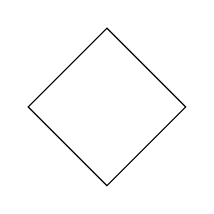
\begin{tikzpicture}
% Define four points
\coordinate (P0) at (1,0);
\coordinate (P1) at (0,1);
\coordinate (P2) at (-1,0);
\coordinate (P3) at (0,-1);
% Draw the diamond
\draw (P0)--(P1)--(P2)--(P3)--cycle;
\end{tikzpicture}

\caption{Using TiKZ for drawing pictures.}
\label{fig:tikz}
\end{figure}
\end{verbatim}

\begin{figure}[h]
\centering

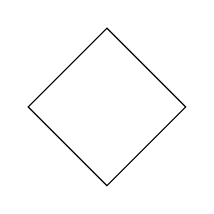
\begin{tikzpicture}
% Define four points
\coordinate (P0) at (0,0);
\coordinate (P1) at (1,0);
\coordinate (P2) at (0,1);
\coordinate (P3) at (-1,0);
\coordinate (P4) at (0,-1);
% Draw the diamond
\draw (P1)--(P2)--(P3)--(P4)--cycle;
\end{tikzpicture}

\caption{Using TiKZ for drawing pictures.}
\label{fig:tikz}
\end{figure}


A great amount of examples are available at \url{http://www.texample.net/tikz/examples/}. 
More information about TiKZ can be found at 
\url{https://en.wikibooks.org/wiki/LaTeX/PGF/TikZ} and 
\url{ftp://ftp.di.uminho.pt/pub/ctan/graphics/pgf/base/doc/pgfmanual.pdf}.

\subsection{PGFPLOTS}

PGFPLOTS provides tools to draw high quality plots, and is based on TiKZ. To use PGFPLOTS in the thesis you need to use \verb|\usepackage{pgfplots}| (in \file{main.tex}).
To guarantee compatibility you need to specify \verb|\pgfplotsset{compat=<version>}|.
You can choose the \verb|version| ().
In this case, it is recommended to choose \verb|newest|. The choice \verb|compat=newest| means "I do not care if my old figures change in appearance after the next version upgrade".

Here it is the \LaTeX{} text for create the graph presented in Figure~\ref{fig:pgfplots}.
\begin{verbatim}
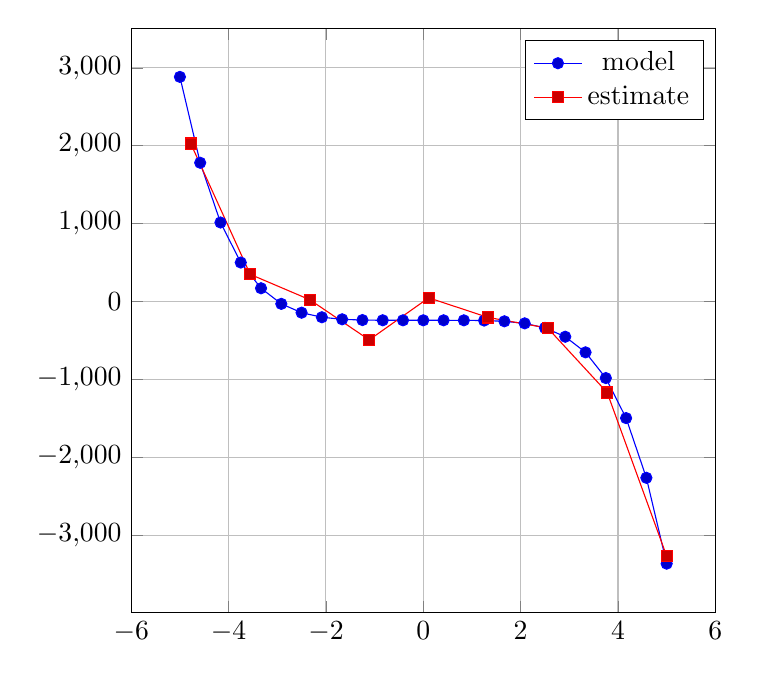
\begin{tikzpicture} 
	\begin{axis}[ height=9cm, width=9cm, grid=major, ] 
		\addplot {-x^5 - 242}; 
		\addlegendentry{model}
		\addplot coordinates { 
			(-4.77778,2027.60977) 
			(-3.55556,347.84069) 
			(-2.33333,22.58953) 
			(-1.11111,-493.50066) 
			(0.11111,46.66082) 
			(1.33333,-205.56286) 
			(2.55556,-341.40638) 
			(3.77778,-1169.24780) 
			(5.00000,-3269.56775) 
		}; 
		\addlegendentry{estimate} 
	\end{axis} 
\end{tikzpicture}
\end{verbatim}

Figure~\ref{fig:pgfplots} shows an example of a graph created using PGFPLOTS functions.

\begin{figure}[h]
\centering
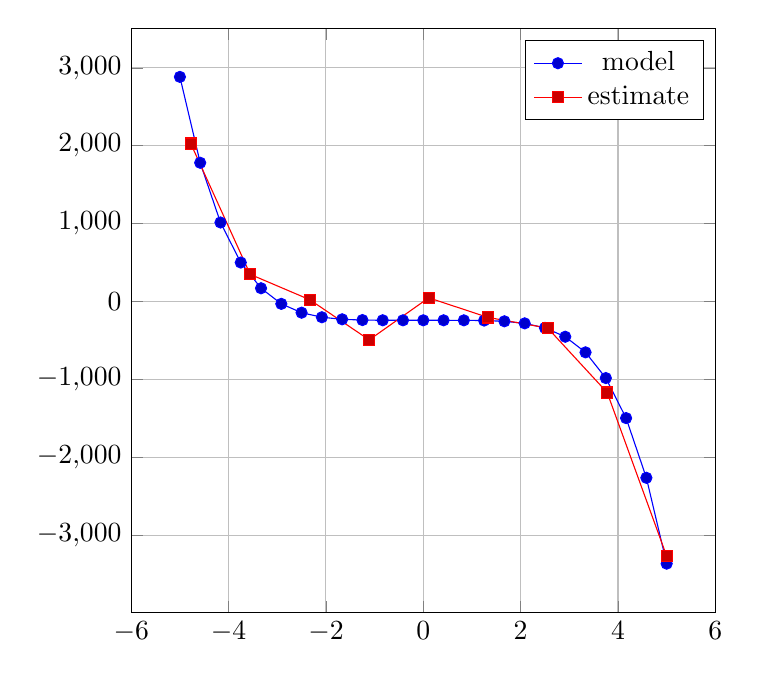
\begin{tikzpicture} 
	\begin{axis}[ height=9cm, width=9cm, grid=major, ] 
		\addplot {-x^5 - 242}; 
		\addlegendentry{model}
		\addplot coordinates { 
			(-4.77778,2027.60977) 
			(-3.55556,347.84069) 
			(-2.33333,22.58953) 
			(-1.11111,-493.50066) 
			(0.11111,46.66082) 
			(1.33333,-205.56286) 
			(2.55556,-341.40638) 
			(3.77778,-1169.24780) 
			(5.00000,-3269.56775) 
		}; 
		\addlegendentry{estimate} 
	\end{axis} 
\end{tikzpicture}
\caption{Using PGFPLOTS for drawing a graph.}
\label{fig:pgfplots}
\end{figure}

A great amount of examples are available at \url{http://pgfplots.sourceforge.net/gallery.html}. 
More information about TiKZ can be found at 
\url{http://pgfplots.sourceforge.net/pgfplots.pdf}.


\section{Handling Acronyms Automatically}
When writing a thesis you need to define acronyms.
According to Wikipedia~\footnote{Accessed in 16 of December of 2015} \textit{"An acronym is an abbreviation used as a word which is formed from the initial components in a phrase or a word."} and
\textit{"Acronyms are used most often to abbreviate names of organizations and long or frequently referenced terms."}.
Typically, an acronym is a pronounceable word, which may already exist or it can be an invented word. 

The use of acronyms imposes two rules: (i) an acronym must be defined in the text during the first appearance of the phrase or word and (ii) the document must have a list of all acronyms alphabetically sorted. In \LaTeX{} this is provided by a package called \verb|\usepackage{glossaries}| that simplifies the use of acronyms. 

Included in this thesis template there is a file called \file{glossary.tex} (in folder \file{frontmatter}), where all acronyms must be written in the form:
\begin{verbatim}
\newacronym{label}{abbrv}{full}
\end{verbatim}
where \verb|label| is the unique label identifying the acronym, \verb|abbrv| is the abbreviated form of the acronym and \verb|full| is the expanded text (word or phrase). This is an example of defining three acronyms:
\begin{verbatim}
\newacronym{RTS}{RTS}{Real-Time System}
\newacronym{GPOS}{GPOS}{General Purpose Operating System}
\newacronym{RTOS}{RTOS}{Real-Time Operating System}
\end{verbatim}

In order to use the features of the \verb|\usepackage{glossaries}|, you have only to use \verb|\gls{label}| command in the text. 
Using this command the acronym will be defined in the first appearance in the text and it will be listed in a list.
For instance, writing this \LaTeX{} text:
\begin{verbatim}
Linux is not a \gls{RTOS} but it is a \gls{GPOS}. 
VxWorks is a \gls{RTOS}, so it is not a \gls{GPOS}.
\end{verbatim}

outputs the following text: 

Linux is not a \gls{RTOS} but it is a \gls{GPOS}. VxWorks is a \gls{RTOS}, so it is not a \gls{GPOS}.

More information about acronyms can be found at 
\url{https://en.wikibooks.org/wiki/LaTeX/Glossary}.

%\chapter{Results}

Here, we consider an example: a simple mechanical system - the inertia wheel pendulum.
\begin{figure}[h]
    \centering
    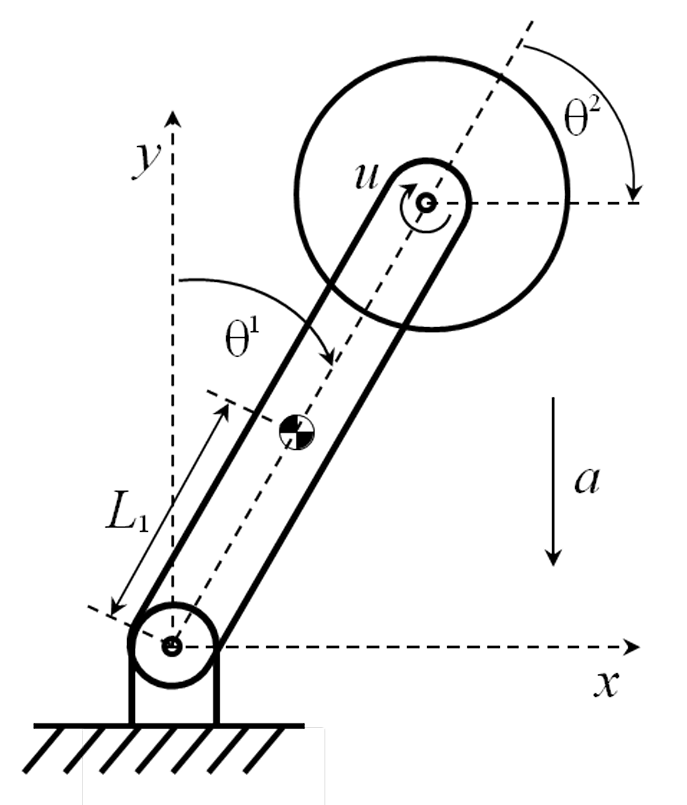
\includegraphics[width=0.35\textwidth]{../Figures/inertia_wheel.png}
    \caption{The inertia wheel pendulum}
    \label{fig:inertia-wheel}
\end{figure}
The equations of motion are given by
\begin{equation}
    \begin{split}
        \mathfrak{m}_{11} \Ddot{\theta}^1 + \mathfrak{m}_{12} \Ddot{\theta}^2 + c^1 = 0\\ 
        \mathfrak{m}_{21} \Ddot{\theta}^1 + \mathfrak{m}_{22} \Ddot{\theta}^2 = u
    \end{split}
\end{equation}

where 
\begin{equation*}
    \begin{split}
        \mathfrak{m}_{11} & = m_d + J_2, \
        \mathfrak{m}_{12} = \mathfrak{m}_{21} = \mathfrak{m}_{22}  = J_2 \\
        m_d  & = L_1^2(m_1 + 4 m_2) + J_1, \
        m_0  = a L_1(m_1 + 2m_2) \\
        c^1  & = -m_0 \sin{\theta^1}
    \end{split}
\end{equation*}

Taking $(\theta^1, \theta^2) = (x_1, x_2)$ and correspondingly $(\dot{\theta}^1, \dot{\theta}^2) = (y_1, y_2)$, we get the following equations:
\begin{equation}
\begin{split}
    \dot{x}_1  & = y_1, \
    \dot{x}_2  = y_2 \\
    \dot{y}_1  & = e_1 + g_1 u, \
    \dot{y}_2  = e_2 + g_2 u
\end{split}
\end{equation}
where 
\begin{equation*}
    \begin{split}
        e_1 = \dfrac{m_0}{m_d}\sin{x_1}, & \ \ g_1 = -\dfrac{1}{m_d} \\
        e_2 = -\dfrac{m_0}{m_d} \sin{x_1}, & \ \ g_2 = \dfrac{m_d + J_2}{m_d J_2}
    \end{split}
\end{equation*}

\section{MF-Linearization}

We will verify $(MD1 - MD3)$ from Proposition~\ref{prop:planar_mech}, since the mechanical system here is a planar mechanical system.

\begin{enumerate}
    \item First, we calculate:
    \begin{equation}
    \begin{split}
        \text{ad}_e g & = 0 - \pmat{
        \frac{m_0}{m_d} \cos{x^1} & 0 \\
        - \frac{m_0}{m_d} \cos{x^1} & 0
        }
        \pmat{
        -\frac{1}{m_d} \\
        \frac{m_d + J_2}{m_d J_2}
        } \\
        & = 
        \pmat{
        \frac{m_0}{m_d^2}\cos{x^1} \\
        -\frac{m_0}{m_d^2}\cos{x^1}
        }
    \end{split}
    \end{equation}
    
    It can be seen that $g$ and $\text{ ad}_e g$ are independent (except at $x_1 = \pm \frac{\pi}{2}$). Thus, $MD1$ is satisfied.
    \item To verify $MD2$,
    \begin{equation}
        \begin{split}
            \nabla_g g & = \left(\dfrac{\partial g_i}{\partial x_j}g_j + \Gamma^i_{jk}g_j g_k \right) \dfrac{\partial}{\partial x_i} = 0 \in \mathcal{E}^0 \\
            \nabla_{\text{ad}_e g} g & = 0 \in \mathcal{E}^0
        \end{split}
    \end{equation}
    which is also verified. 
    \item Lastly, for $MD3$,
    \begin{equation}
    \label{eq:md3-1}
        \begin{split}
            \nabla^2_{g, \text{ad}_e g} \text{ad}_e g = \nabla^2_{\text{ad}_e g, g} \text{ad}_e g = \pmat{
            \frac{m_0^2}{m_d^5}\cos^2{x_1} \\
            - \frac{m_0^2}{m_d^5} \cos^2{x_1}
            }
        \end{split}
    \end{equation}
    and,
    \begin{equation}
    \label{eq:md3-2}
        \begin{split}
            \nabla^2_{\text{ad}_e g, g} \text{ad}_e g & = \nabla_{\text{ad}_e g} \nabla_g \text{ad}_e g - \nabla_{\nabla_{\text{ad}_e g} g} \text{ad}_e g \\
            & = \pmat{
            \frac{m_0^2}{m_d^5}\cos^2{x_1} \\
            - \frac{m_0^2}{m_d^5} \cos^2{x_1}
            }
        \end{split}
    \end{equation}
    
\end{enumerate}
 
Thus, we have:
\begin{equation}
    \nabla^2_{g, \text{ad}_e g} \text{ad}_e g - \nabla^2_{\text{ad}_e g, g} \text{ad}_e g = 0 \in \mathcal{E}^0
\end{equation}
Therefore, all the conditions $(MD1 - MD3)$ are satisfied, and the given system is $MF$-Linearizable.

We have the diffeomorphism $\Phi(x,y) = \left( \varphi(x), D\varphi(x)y\right)$, which is given by:
\begin{equation}
\begin{split}
        \tilde{x}_1  = \dfrac{m_d+J_2}{J_2}x_1 + x_2, \ 
        \tilde{x}_2  = \dfrac{m_0}{J_2}\sin{x_1} \\
        \tilde{y}_1  = \dfrac{m_d+J_2}{J_2}y_1 + y_2,\
        \tilde{y}_2  = \dfrac{m_0}{J_2}\cos{x_1}y_1
\end{split}
\end{equation}

Taking $\tilde{\text{x}} = \pmat{\tilde{x}_1 & \tilde{x}_2 & \tilde{y}_1 & \tilde{y}_2 }^T$, such that the linearized equations become:
% A = [[0 0 1 0]; [0 0 0 1]; [0 1 0 0]; [0 0 0 0]];
% B = [0; 0; 0; 1];
\begin{equation}
    \dfrac{d}{dt} \tilde{\text{x}}
    = A \tilde{\text{x}} + B \tilde{u}
\end{equation}

Here, the matrices $A = \pmat { 0 & 0 & 1 & 0 \\ 0 & 0 & 0 & 1 \\ 0 & 1 & 0 & 0 \\ 0 & 0 & 0 & 0 }$, $B = \pmat{0 \\ 0 \\ 0 \\ 1}$ and
$\tilde{u} = \psi (x, y, u)$ is the auxiliary control, such that:
\begin{equation}
    \tilde{u} = -\dfrac{m_0}{J_2} \sin{x_1}y_1^2 + \dfrac{m_0^2}{2m_dJ_2}\sin{2x_1} - \dfrac{m_0}{m_d J_2} \cos{x_1} u
\end{equation}


\section{Stabilization}
We use the pole placement technique to obtain a control gain matrix $K$, such that $\tilde{u} = - K \tilde{x}$.

Let us choose the poles of the closed-loop system to be:
\begin{equation}
    \lambda = -10, -20, -30, -40
\end{equation}

Correspondingly, we obtain $K = \bmat{240000 & 3500 & 50000 & 100}$

We denote $\text{x} = \bmat{x_1 & x_2 & y_1 & y_2}^T$ to get:
\begin{equation}\label{eq:feedback}
    \dfrac{d}{dt} \text{x}
    = \left( A - B K \right) \text{x}
\end{equation}

\section{Discretization}
We have the system in the form 

\[ \dot{\text{x}} = (A-BK)\text{x} = F(\text{x}) \] 

Let $h$ denote a (fixed) sampling time and $h' = \dfrac{h}{2}$. We utilize the symmetric discretization formulated in Section~\ref{sec:retr-intro}:
\[
F(\text{x}_k; h/2) = F(\text{x}_{k+1}; -h/2)
\]
$$
\text{x}_k + h' (A-BK) \text{x}_k = \text{x}_{k+1} - h'(A-BK) \text{x}_{k+1} 
$$
\begin{equation}
    \therefore \text{x}_{k+1} = {(I - h'(A-BK))}^{-1}(I + h'(A-BK)) \text{x}_k
\end{equation}

\section{Simulations}
We use the following parameters from~\cite{nowicki} and~\cite{SPONG20011845}:
\begin{equation}
\begin{split}
    L_1 & = 0.063 \ [m] \\
    m_1 & = 0.02 \ [kg] \\
    m_2 & = 0.3 \ [kg] \\
    J_1 & = 47 \cdot 10^{-6} \ [kg \cdot m^2] \\
    J_2 & = 32 \cdot 10^{-6} \ [kg \cdot m^2] \\
    a & = 9.81 \ [m s^{-2}] \\
    m_0 & = 0.3832 \ [kg \cdot m^2 s^{-2}] \\
    m_d & = 49 \cdot 10^{-4} \ [kg \cdot m^2] 
\end{split}
\end{equation}

% \begin{table}[h]
%     \centering
%     \begin{tabular}{|ccc|}
%     \hline
%         $L_1 = 0.063 \ m$ & $m_1 = 0.02 \ kg$ & $m_2 = 0.3 \ kg$ \\
%         $J_1 = 47 \times 10^{-6} \ kg m^2$ & $J_2 = 32 \times 10^{-6} \ kg m^2$ & $a=9.81 \ m s^{-2}$ \\  
%         \multicolumn{3}{|c|}{
%         $m_0 = 0.3832 \ kg m^2 s^{-2}$ \ \ \ \ $m_d = 49 \times 10^{-4} kg m^2$ } \\
%     \hline
%     \end{tabular}
%     \caption{Parameters for simulations}
%     \label{tab:params}
% \end{table}
% \vspace{-0.65cm}
The comparison results between the proposed discretization scheme and ODE45 for the system, for a sampling time of $h = 0.01$, and initial conditions $\theta^1(0) = \frac{\pi}{4}, \theta^2(0) = \dot{\theta}^1(0) = \dot{\theta}^2(0) = 0$ are shown in Figure \ref{fig:sim-results}. The errors are plotted in Figs.~\ref{fig:e1-ed1},~\ref{fig:e2-ed2}.
% In Figure \ref{fig:perc-errors}, we compare the (percentage) relative error $100 \times \frac{\lVert e(t_k) \rVert}{\lVert x(t_k) \rVert}$.}
\begin{figure}[ht]
  \begin{center}
    \begin{tikzpicture}
      \begin{axis}[
          width=0.8\linewidth,
          height=0.6\linewidth,
          xlabel=$t_k (s)$,
          ylabel=$\theta_1$ (rad),
          xmin = 0, xmax = 1,
          axis x line* = none,
          axis y line* = left,
          legend style={at={(0.61,0.97)}}
        ]
        \addplot[mark=none, red, ultra thick] table[x=t,y=theta1, col sep=comma]{../Data/inertia_pendulum/states_original.csv};
        \addlegendentry{$\theta_{1,k}$}
        \addplot [mark=none, black, dashed, ultra thick]
        table[x=t,y=theta1,col sep=comma]{../Data/inertia_pendulum/states_ode45.csv}; 
        \addlegendentry{$\theta_1(t_k)$}
      \end{axis}
    \begin{axis}[
          width=0.8\linewidth,
          height=0.6\linewidth,
          xlabel=$t_k (s)$,
          ylabel=$\theta_2$ (rad),
          xmin = 0, xmax = 1,
          axis x line* = none,
          axis y line* = right,
          legend pos=north east
        ]
        \addplot[mark=none, blue, ultra thick] table[x=t,y=theta2, col sep=comma]{../Data/inertia_pendulum/states_original.csv};
        \addlegendentry{$\theta_{2,k}$}
        \addplot [mark=none, green, dashed, ultra thick]
        table[x=t,y=theta2,col sep=comma]{../Data/inertia_pendulum/states_ode45.csv};
        \addlegendentry{$\theta_2(t_k)$}
      \end{axis}  
    \end{tikzpicture}
    \caption{System states $x_k$ for symmetric discretization plotted against exact discretization (ODE45) $x(t_k)$ for $t_k \in [0, 1]$}
    \label{fig:sim-results}
  \end{center}
\end{figure}

\begin{figure}[ht]
    \begin{center}
      \begin{tikzpicture}
      \begin{axis}[
            width=0.8\linewidth,
            height=0.6\linewidth,
            xlabel=$t_k (s)$,
            ylabel=$|| e(k) ||$,
            xmin = 0, xmax = 1,
            axis x line* = none,
            axis y line* = left,
            legend pos=north east
          ]
          \addplot[mark=none, blue, thick] table[x=t,y=e1, col sep=comma]{../Data/inertia_pendulum/error_norms.csv};
          \addlegendentry{$\lVert \theta_{1,k}-\theta_1(t_k) \rVert$}
        \end{axis}  
        \begin{axis}[
            width=0.8\linewidth,
            height=0.6\linewidth,
            xlabel=$t_k (s)$,
            ylabel=$||\dot{e}(k)||$,
            xmin = 0, xmax = 1,
            axis x line* = none,
            axis y line* = right,
            legend style={at={(0.97,0.77)}}
          ]
          \addplot[mark=none, red, thick] table[x=t,y=ed1, col sep=comma]{../Data/inertia_pendulum/error_norms.csv};
          \addlegendentry{$\lVert \dot{\theta}_{1,k}-\dot{\theta}_1(t_k) \rVert$}
        \end{axis}  
      \end{tikzpicture}
      \caption{Magnitude of error norm for $\theta_1$ and $\dot{\theta}_1$}
      \label{fig:e1-ed1}
    \end{center}
  \end{figure}

  \begin{figure}[ht]
  \begin{center}
    \begin{tikzpicture}
    \begin{axis}[
          width=0.8\linewidth,
          height=0.6\linewidth,
          xlabel=$t_k (s)$,
          ylabel=$|| e(k) ||$,
          xmin = 0, xmax = 1,
          axis x line* = none,
          axis y line* = left,
          legend pos=north east
        ]
        \addplot[mark=none, blue, thick] table[x=t,y=e2, col sep=comma]{../Data/inertia_pendulum/error_norms.csv};
        \addlegendentry{$\lVert \theta_{2,k}-\theta_2(t_k) \rVert$}
      \end{axis}  
      \begin{axis}[
          width=0.8\linewidth,
          height=0.6\linewidth,
          xlabel=$t_k (s)$,
          xmin = 0, xmax = 1,
          axis x line* = none,
          axis y line* = right,
          legend style={at={(0.97,0.77)}}
        ]
        \addplot[mark=none, red, thick] table[x=t,y=ed2, col sep=comma]{../Data/inertia_pendulum/error_norms.csv};
        \addlegendentry{$\lVert \dot{\theta}_{2,k}-\dot{\theta}_2(t_k) \rVert$}
      \end{axis}  
    \end{tikzpicture}
    \caption{Magnitude of error norm for $\theta_2$ and $\dot{\theta}_2$}
    \label{fig:e2-ed2}
  \end{center}
\end{figure}



% \begin{figure}[ht]
%   \begin{center}
%     \begin{tikzpicture}
%       \begin{axis}[
%           width=0.8\linewidth,
%           height=0.6\linewidth,
%           xlabel=$t_k (s)$,
%           ylabel=$x$ (m),
%           xmin = 0, xmax = 10,
%           axis x line* = none,
%           axis y line* = left,
%           legend style={at={(0.61,0.97)}}
%         ]
%         \addplot[mark=none, red, ultra thick] table[x=t,y=x, col sep=comma]{../Data/tora/states_original.csv};
%         \addlegendentry{$x_{k}$}
%         \addplot [mark=none, black, dashed, ultra thick]
%         table[x=t,y=x,col sep=comma]{../Data/tora/states_ode45.csv}; 
%         \addlegendentry{$x(t_k)$}
%       \end{axis}
%     \begin{axis}[
%           width=0.8\linewidth,
%           height=0.6\linewidth,
%           xlabel=$t_k (s)$,
%           ylabel=$\theta$ (rad),
%           xmin = 0, xmax = 10,
%           axis x line* = none,
%           axis y line* = right,
%           legend pos=north east
%         ]
%         \addplot[mark=none, blue, ultra thick] table[x=t,y=theta, col sep=comma]{../Data/tora/states_original.csv};
%         \addlegendentry{$\theta{k}$}
%         \addplot [mark=none, green, dashed, ultra thick]
%         table[x=t,y=theta,col sep=comma]{../Data/tora/states_ode45.csv};
%         \addlegendentry{$\theta(t_k)$}
%       \end{axis}  
%     \end{tikzpicture}
%     \caption{System states $x_k$ for symmetric discretization plotted against exact discretization (ODE45) $x(t_k)$ for $t_k \in [0, 10]$}
%     \label{fig:sim-2-results}
%   \end{center}
% \end{figure}

% \begin{figure}[ht]
%   \begin{center}
%     \begin{tikzpicture}
%     \begin{axis}[
%           width=0.8\linewidth,
%           height=0.6\linewidth,
%           xlabel=$t_k (s)$,
%           ylabel=$|| e(k) ||$,
%           xmin = 0, xmax = 10,
%           axis x line* = none,
%           axis y line* = left,
%           legend pos=north east
%         ]
%         \addplot[mark=none, blue, thick] table[x=t,y=e1, col sep=comma]{../Data/tora/error_norms.csv};
%         \addlegendentry{$\lVert x_{k}-x(t_k) \rVert$}
%       \end{axis}  
%       \begin{axis}[
%           width=0.8\linewidth,
%           height=0.6\linewidth,
%           xlabel=$t_k (s)$,
%           ylabel=$||\dot{e}(k)||$,
%           xmin = 0, xmax = 10,
%           axis x line* = none,
%           axis y line* = right,
%           legend style={at={(0.97,0.77)}}
%         ]
%         \addplot[mark=none, red, thick] table[x=t,y=ed1, col sep=comma]{../Data/tora/error_norms.csv};
%         \addlegendentry{$\lVert \dot{x}_{k}-\dot{x}(t_k) \rVert$}
%       \end{axis}  
%     \end{tikzpicture}
%     \caption{Magnitude of error norm for $x$ and $\dot{x}$}
%     \label{fig:e1-ed1-2}
%   \end{center}
% \end{figure}

% \begin{figure}[ht]
%   \begin{center}
%     \begin{tikzpicture}
%     \begin{axis}[
%           width=0.8\linewidth,
%           height=0.6\linewidth,
%           xlabel=$t_k (s)$,
%           ylabel=$|| e(k) ||$,
%           xmin = 0, xmax = 10,
%           axis x line* = none,
%           axis y line* = left,
%           legend pos=north east
%         ]
%         \addplot[mark=none, blue, thick] table[x=t,y=e2, col sep=comma]{../Data/tora/error_norms.csv};
%         \addlegendentry{$\lVert \theta_{k}-\theta(t_k) \rVert$}
%       \end{axis}  
%       \begin{axis}[
%           width=0.8\linewidth,
%           height=0.6\linewidth,
%           xlabel=$t_k (s)$,
%           xmin = 0, xmax = 10,
%           axis x line* = none,
%           axis y line* = right,
%           legend style={at={(0.97,0.77)}}
%         ]
%         \addplot[mark=none, red, thick] table[x=t,y=ed2, col sep=comma]{../Data/tora/error_norms.csv};
%         \addlegendentry{$\lVert \dot{\theta}_{k}-\dot{\theta}(t_k) \rVert$}
%       \end{axis}  
%     \end{tikzpicture}
%     \caption{Magnitude of error norm for $\theta$ and $\dot{\theta}$}
%     \label{fig:e2-ed2-2}
%   \end{center}
% \end{figure}
%\input{ch5/chapter5}


%----------------------------------------------------------------------------------------
%	BIBLIOGRAPHY
%----------------------------------------------------------------------------------------

\printbibliography[heading=bibintoc]

%----------------------------------------------------------------------------------------
%	THESIS CONTENT - APPENDICES
%----------------------------------------------------------------------------------------
% Include the appendices of the thesis as separate files from the Appendices folder
% Uncomment the lines as you write the Appendices
\begin{appendices}

% % Appendix A

\chapter{Appendix Title Here} % Main appendix title

\label{AppendixA} % For referencing this appendix elsewhere, use \ref{AppendixA}

Write your Appendix content here.
%\input{appendices/appendixB}
%\input{appendices/appendixC}

\end{appendices}
%----------------------------------------------------------------------------------------

\end{document}
